%
% File: chap04.tex
% Description: Investigation Proposal chapter 
%
\let\textcircled=\pgftextcircled
\chapter{Research Proposal}
\label{chap:RelatedWork}
\initial{I}n this chapter the investigation proposal is presented. The problem definition, justification, hypothesis, objectives, scope and limitation, and testing methodology are explained. 

\section{Problem Definition}
\label{sec:problemDefinition}
Redundant Multi-Threading is a replication-based technique to detect soft errors. The original application code is duplicated in two threads, the producer or leading thread and the consumer or trailing thread. Both threads execute almost the same code and every time a value needs to be checked, there is data exchange from the producer to the consumer and or vice versa. The latter thread, performs additional checks in order to compare both values and be sure that no soft error has happened. In such schemes, communication between threads happens frequently and that represents the main performance bottleneck of such solutions.

There are 3 types of communication patterns in RMT solutions, synchronous, asynchronous and semi-synchronous. In the first one, the leading thread must wait for the trailing thread confirmation on every memory operation, making the performance overhead unmanageable. RMT schemes with asynchronous communication patterns try to minimize the data exchange between the two threads. They let the producer make forward progress all the time without a check from the consumer. When there are no volatile memory accesses such schemes provides enough soft-error-detection with low performance overhead \cite{mitropoulou2016comet}. However on the other hand, when there are volatile memory accesses, an asynchronous communication pattern does not offer sufficient protection. RMT approaches with semi-synchronous communication patterns take into account volatile memory accesses and still try to provide low inter-thread data exchanging. The basic idea is to allow the leading thread continue without a proof of correctness as much as possible, while delivering safe execution of volatile memory access. 

Although there are several variations of a Redundant Multi-Threading soft error detection technique, in general they incurs a lot of performance overhead because of the highly frequent inter-thread communication. 

\section{Justification}
\label{sec:justification}

\subsection{Volatile Variable Accesses}
\label{subsubsec:volatileAccesses}
Several authors \cite{mitropoulou2016comet} \cite{wang2007compiler} \cite{zhang2012daft}  claim that applications have few volatile variable accesses and that RMT with synchronous communication pattern is unrealistic because it adds so much performance overhead. In COMET the authors even decide not to protect at all against such instructions. But we have found that volatile variable accesses are not too uncommon. Many real HPC applications use programming models like MPI or OpenMP, where data needs to be transfered between nodes or threads regularly. Each one of these function calls includes at least one volatile memory access that should be confirmed to be correct before execution. As an example of this, there are several programs included in the Mantevo benchmark project \footnote{https://mantevo.org/}. The Mantevo project has a set of mini applications (kernels) that are representative in the HPC programs. These small software examples perform the most common work that HPC real software do as well \cite{heroux2009improvingMantevo}. For example, the HPCCG mini app is described as follows: 

``\emph{Many engineering applications require the implicit solution of a nonlinear system of equations where the vast majority of time as problem size increases is spent in some variation of a conjugate gradient solver. As a result, any miniapp focusing on this area will necessarily have a conjugate gradient solver as the dominant computational kernel. MiniFE or HPCCG is a miniapp that mimics the finite element generation, assembly and solution for an unstructured grid problem}''

Such software does represent a lot of engineering HPC applications. In this case the problems is solved with an iterative algorithm that approximates the solution. If the application is executed with MPI, on every round of the loop that data is refined there is a send/receive instruction to neighbors nodes and every one of these communication instructions represents at least one volatile store. On the other hand, if it is run in a single machine with multiple threads, on every iteration there is also communication among threads; which again are volatile stores. 

Another example is MiniXyce: Electrical Circuits, also a miniapp from the Mantevo project. It is explained as follows:

``\emph{The MiniXyce application is a miniature version of Xyce, a circuit simulation application. Circuit simulation is the cornerstone of the electrical design automation (EDA) industry, and is a crucial part of commercial electrical design. Like most circuit simulation tools, MiniXyce is based on a modified nodal analysis (MNA) formulation, resulting in Kirchoff Current Laws (KCL) being enforced across a potentially arbitrary network. The resulting system of differential-algebraic equations (DAEs) is solved implicitly using Newton- based methods. Traditional circuit codes have almost exclusively relied upon direct matrix solvers, but preconditioned GMRES is the method of choice for parallel simulation}''

MiniXyce is an MPI program which firstly performs work creating the system of DAEs, in which there is some communication with the neighbors through MPI calls. Once the system has been built, it is solved with the generalized minimal residual method (usually abbreviated GMRES), which again is an iterative algorithm that approximates the solution every time. Here at each round of the loop, after plenty of work is performed, including several sparse-matrix-vector-product, data is exchanged among neighbors through more MPI calls.

Such mini applications serve as an example to demonstrate that volatile variable accesses are not that uncommon in HPC software and therefore any Redundant Multi-Threading mechanism should be aware of them. Therefore we believe that a safe approach is to have a solution with semi-synchronous communication pattern, that on every volatile memory access must allow the trailing thread to catch up with the leading one, in order to provide confirmation that no soft error has happened; similar to the solution provided by \cite{wang2007compiler}. As said before, this scheme also has high inter-thread communication costs, which we believe can be mitigated with the use of Hyper-Threading. Since hyper-threads share the cache L1, data communication between them is faster that having the threads on different cores. 

\subsection{Redundant Multi-Threading with Hyper-Threads}
\label{subsec:redundantHyper-threading}

We only know of one experiment that has tested how hyper-threads behave in a Redundant Multi-Threading technique\cite{wang2007compiler}. In such tests, further explained in Section \ref{subsec:useOfHyperThreading}, the hyper-thread option came in really close, even better in some cases, to the best configuration (having two threads in the same cluster sharing the L4 cache). Also the last option of two threads in different clusters not sharing a L4 cache behave significantly worse than the two other options. We believe the following reasons justify a more detailed investigation of Hyper-Threading in Redundant Multi-Threading approaches:

\begin{itemize}
\item Such experiments were performed a long time ago (more than 10 years ago), in which some implementation details of Hyper-Threading may have been improved by Intel.
\item The specific physical characteristics of the test machine cannot be generalized to all supercomputers.
\item The technique tested was not specifically designed to run on hyper-threads, therefore there might be some modifications that might decrease the overhead.
\item The overall time performance of the technique with hyper-threads does not necessarily has to be better, compared against threads on different cores, to justify its use. Hyper-Threads run on a single core, therefore if a hyper-threaded version of the technique performs similar to threads on different cores, means that the resource utilization overhead of the system can be significantly improved. 
\end{itemize}

%% ----------------------------------------------------------------------------------------------------------------------------------------
%% ----------------------------------------------------------------------------------------------------------------------------------------
\section{Hypothesis}
\label{sec:Hypothesis}

Using hyper-threads, instead of threads on two cores, on a redundant multi-threading soft-error detection technique with semi-synchronous communication pattern, halves the compute-core utilization while incurring at most 20\% time overhead. 

\section{Objectives}
\label{sec:objectives}

\subsection{General Objective}
\label{subsec:generalObjective}
The main objective of this thesis is to create a Redundant Multi-Threading approach (called Redundant Hyper-Threading) with semi-synchronous communication pattern to reduce compute-core utilization without significantly degrading performance.

\subsection{Specific Objectives}
\label{subsec:specificObjective}

\begin{enumerate}
\item Design the Redundant Hyper-Threading technique exploiting Intel Hyper-Threading infrastructure.
\item Implement the Redundant Hyper-Threading technique in the C programming language. 
\item Evaluate the performance of the Redundant Hyper-Threading technique and compare to the same strategy with threads on different cores. 
\end{enumerate}

\section{Scope and Limitations}
\label{sec:scopeAndLimitations}
The current thesis focus only soft error detection, specifically on a Redundant Multi-Threading approach. Since checkpointing techniques have been commonly used for soft error correction, we believe our scheme can easily be further combined with such a technique in order to provide complete soft error management. 

\subsection{Restrictions and Assumptions}
\label{subsec:restrictionsAndAssumptions}
It is assumed main memory is already protected by mechanisms like ECC against bit flips. Also, only one of these faults is expected to happen per execution of the application (a Single Event Upset, SEU). Both assumptions are commonly made in the literature \cite{calhoun2017towards} \cite{kuvaiskii2016haft} \cite{mitropoulou2016comet} \cite{wang2007compiler} \cite{zhang2012daft}. 

%though that does not mean that the technique is useless in the case where more than one transient fault occurs. In fact, most of the times it will detect an error and report it. Only in very unlikely cases, such as where two bit flips modify the values being compared in exactly the same bit, so both modified values end up being exactly the same

\section{Test Methodology}
\label{sec:testMethodology}
The final software and experiments will be run in different machines on the Grid'5000. Grid'5000 is a large-scale and versatile testbed for experiment-driven research in all areas of computer science, with a focus on parallel and distributed computing including Cloud, HPC and Big Data. Next are some features about Grid'5000: \footnote{https://www.grid5000.fr/mediawiki/index.php/Grid5000:Home}

\begin{itemize}
\item provides access to a large amount of resources: 1000 nodes, 8000 cores, grouped in homogeneous clusters, and featuring various technologies: 10G Ethernet, Infiniband, GPUs, Xeon PHI.
\item highly reconfigurable and controllable: researchers can experiment with a fully customized software stack thanks to bare-metal deployment features, and can isolate their experiment at the networking layer
\item advanced monitoring and measurement features for traces collection of networking and power consumption, providing a deep understanding of experiments
\item designed to support Open Science and reproducible research, with full traceability of infrastructure and software changes on the testbed
\end{itemize}

In order to try to provide HPC representative results with our experiments, we will be using applications part of the Mantevo Project (already mentioned in Section \ref{sec:justification}). Such applications are small examples of real HPC software. There will be 3 versions of each mini-app. A baseline, which represent the program executed without soft-error detection. Two other version that will include soft-error detection, and are therefore expected to be slower. A core-threaded-version, with our Redundant Multi-Threading technique in which the leading and trailing thread will be pinned to different cores. Lastly, a hyper-threaded-version, with our Redundant Multi-Threading technique, in which both threads will be pinned to the same core, hence exploiting the hyper-threading capabilities available in the chip. 

In order to have a better understanding of the technique performance, we believe utilizing hardware counters is a good alternative. For that, tools such as \textit{perf} offer easy ways to accomplish this. Performance counters are CPU hardware registers that count hardware events such as instructions executed, cache-misses suffered, or branches mispredicted. They form a basis for profiling applications to trace dynamic control flow and identify hotspots. perf provides rich generalized abstractions over hardware specific capabilities. Among others, it provides per task, per CPU and per-workload counters, sampling on top of these and source code event annotation \footnote{https://perf.wiki.kernel.org/index.php/Main\_Page}.

% An anova will be most likely be used.

%\subsection{Fault Injection}
%\label{subsec:faultInjection}
%
%Since transient faults are not easy to predict, in order to test the reliability of a soft error detection technique it is necessary to %simulate these kind of faults. 

%\begin{figure}[h]
%	\centering
%	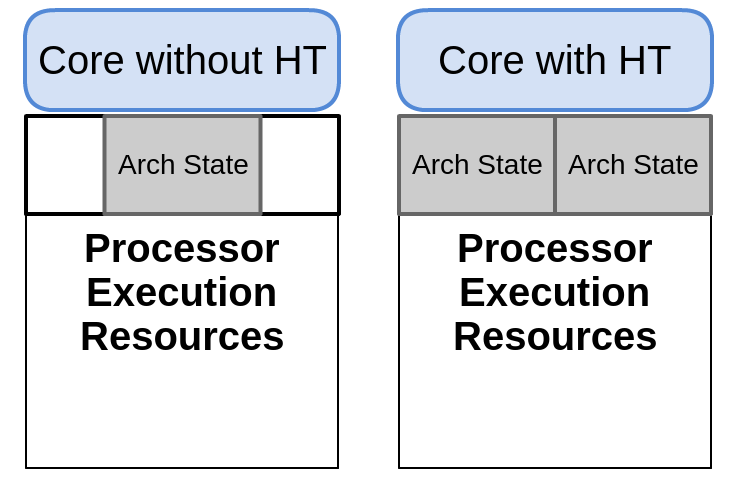
\includegraphics[height=0.35\textheight]{images/Hyper-Threading.png}
%	\mycaption[Core with and without Hyper-Threading]{Core with and without %Hyper-Threading}
%	\label{fig:Hyper-Threading}
%\end{figure}









